
\section{Radiation Pressure Noise}
\label{sec:V}
Another advantage of radiation pressure control, compared to a classical approach based on photo detection and feedback, is its fundamental noise limit. Unlike in the classical approach, the shot noise and other sensing noises %from detecting a potentially small sample of the beam 
never enter a radiation-pressure-based feedback loop. Even though technical laser noise is typically bigger in the simple cavity setup discussed in this paper, the only fundamental noise source of the scheme is quantum radiation pressure noise. In this section we give the full expression for radiation pressure noise in the case of a dual-carrier stable optical spring.

First, we note that as long as we are interested in frequencies much smaller than the any of the features in the detuned cavity transfer function, the radiation pressure noise is relatively simple. If we also assume that the end mirror has a reflectivity of 1, the one-sided ($f\ge0$) radiation-force amplitude spectral noise density is given by
\begin{eqnarray}
\label{eqn:simpleRPN}
S_F (f) = \frac{2}{c} G \sqrt{2 \hbar \omega P_{\rm in}}
\end{eqnarray}
where $G$ is the power gain of the cavity in the detuned configuration, and $P_{\rm in}$ is the power of the shot noise limited beam entering the cavity.
Equation \ref{eqn:simpleRPN} is valid for carrier and subcarrier separately.
Note that this equation does not hold if the end mirror has a finite transmissivity, as quantum fluctuations entering from that port will also contribute to the intra-cavity shot noise. In the case of a critically coupled cavity, this will result in an increase of the intra-cavity radiation-force amplitude spectral noise density by exactly a factor of 2.

To calculate the exact expression for the radiation pressure noise induced cavity fluctuations, we first realize that we can calculate the radiation-force amplitude spectral noise for a static cavity, and then compute the response of the dual-carrier optical spring system to that driving force. This yields the correct answer up to first order in the size of the quantum fluctuations. For the calculation we track the quantum vacuum fluctuations entering at both ports of the cavity. It is useful to introduce a function $F$:
\begin{eqnarray}
\label{eqn:RPNfunction}
F(f) = F\left(\frac{\Omega + \delta + \omega_{res}}{2 \pi}\right) =& \frac{1}{1-XY^2}  \\ =& \frac{1}{1-r_1r_2e^{-2 i \delta\tau}e^{-2 i \Omega\tau}}
\end{eqnarray}
The amplitude build-up factors for fluctuations at frequency $f$ entering through the input coupler (1) and the end mirror (2) thus are
\begin{eqnarray}
\label{eqn:RPNfunction12}
 t_1 F(f) \,\,\, {\rm and} \,\,\ r_1 t_2 F(f), 
\end{eqnarray}
where we already dropped the one-way propagation factor because it drops out in the radiation force noise calculation below. 
We can now introduce the notation $F_0=F(f_0)$, $F_+=F(f_0+f)$ and $F_-=F(f_0-f)$. We then get the following expression for the one-sided radiation-force power spectral density for either carrier or sub-carrier.
\begin{eqnarray}
\label{eqn:RPN_P}
S_F (f) = \frac{2}{c} S_P (f) \,\,\,\,\,\, {\rm and}
\end{eqnarray}
\begin{eqnarray}
\label{eqn:RPN}
|S_P (f)|^2 =   \hbar \omega P_0 t_1^2|F_0|^2 (t_1^2 \!\!+\! r_1^2t_2^2)( |F_+|^2 \!\!+\!  |F_-|^2)
\end{eqnarray}
Here $P_0$ is the entering carrier power, and $f_0$ is its frequency. We can see that we recover equation \ref{eqn:simpleRPN} in the limit $t_2 \rightarrow 0$ and $G/t_1^2=|F_0|^2=|F_+|^2=|F_-|^2$. The resulting force noise from carrier and sub-carrier for the cavity A in the example above is plotted in Fig.\ref{fig:RFASD} (\emph{top}).
\begin{figure}[htbp]
	\centering
		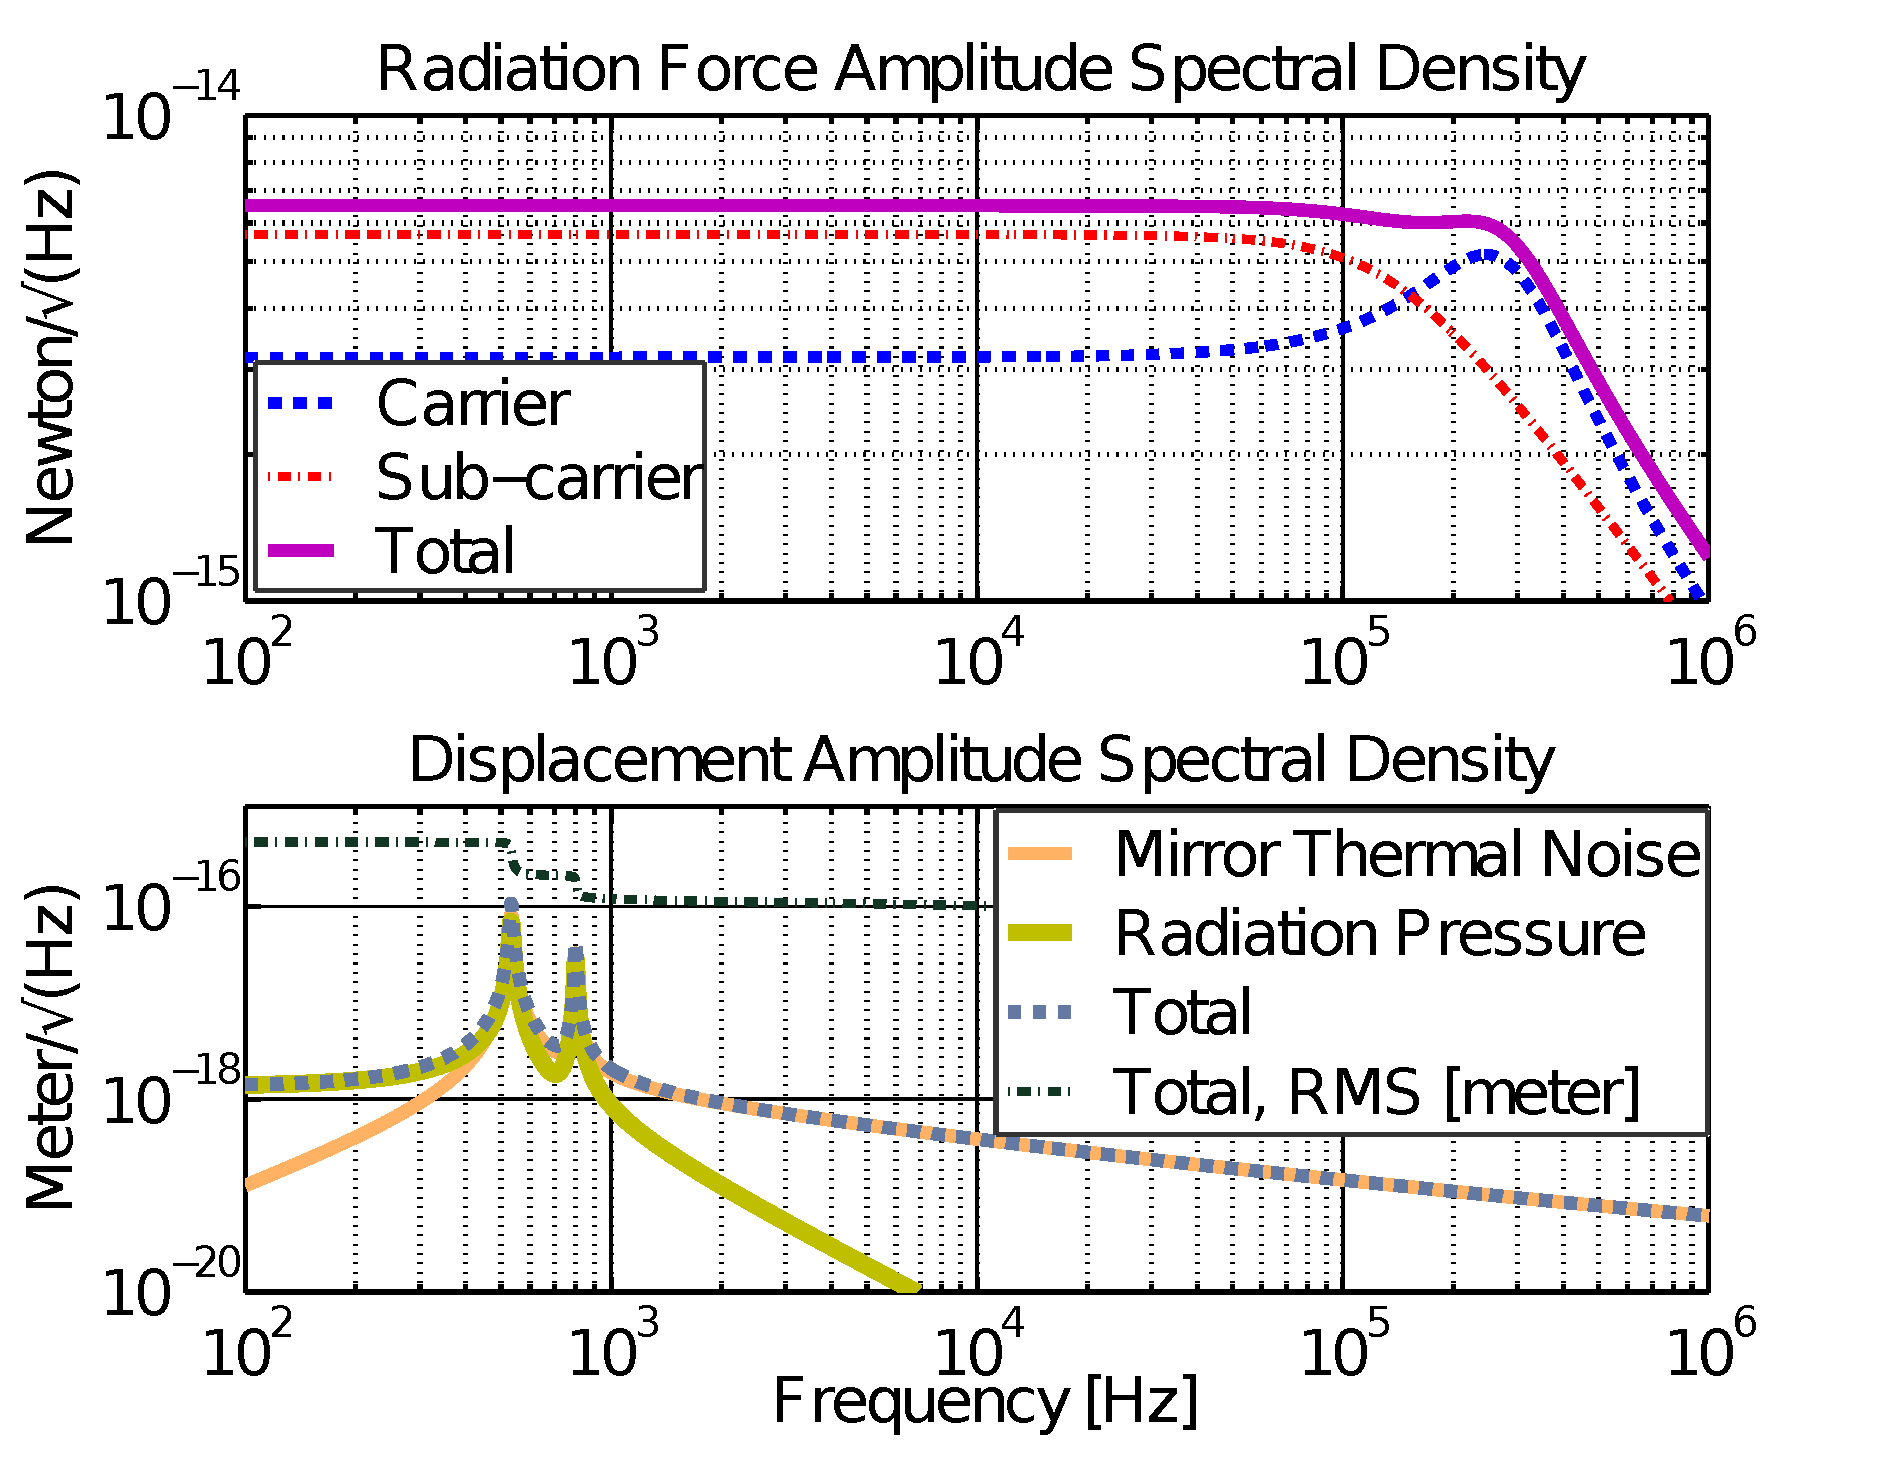
\includegraphics[width=8.5cm]{./figures/trap_radPresA_paper2.pdf}
	\caption[Radiation Pressure Noise]{
        (\emph{Top}) Radiation force amplitude spectral density for the dual-carrier optical spring used in beam A of the above example. The sub-carrier dominates the noise at low frequency, but the higher-power carrier contributes more at high frequencies. Also note that if we choose the same free spectral range for the two carriers, there would be an additional beat note at the difference frequency of $310~{\rm kHz}$. (\emph{Bottom})  Radiation pressure and thermal noise displacement amplitude spectral density. The radiation pressure noise is calculated using the opto-mechanical response given in equation \ref{eqn:closedloop_tf}. The thermal noise is based on a theoretical calculation described in \cite{Saulson90}, \cite{Ballmer13}. Since seismic and suspension thermal noise depend on the experimental implementation, they are not shown, but they would also be suppressed by the optical spring closed loop response. The residual RMS motion due to the shown noise sources is less than $10^{-3}$ picometer. With the total RMS motion smaller than the 20 picometer stability band shown in Fig.\ref{fig:stability_region}, the two cavities will remain locked purely due to the radiation pressure trapping force.}
	\label{fig:RFASD}
\end{figure}

Next we calculate the response of the coupled opto-mechanical system to this driving force, using the following closed loop transfer function obtained from equations \ref{eq:MF} and \ref{eq:HX}:

\begin{eqnarray}
\label{eqn:closedloop_tf}
x = {M}({1-HM})^{-1}F
\end{eqnarray}

Above the optical spring resonances this leads to a $1/f^2$ fall-off of the displacement noise, as expected for radiation pressure noise. Meanwhile below the resonance, due to the closed loop suppression, we will have a flat displacement noise. %at a level of $S_x(f) ~ S_F(f)/K_{OS}$. 
Fig.\ref{fig:RFASD} bottom illustrates this in the case of the two-dimensional angular trap discussed above.

Finally we compare the resulting displacement noise to a classical photo-detection feedback control scheme with similar control bandwidth and control loop shape. If such a system is able to detect all availabe power and has no other dominating sensing noise sources, it can at best achieve a shot noise sensitivity of 
\begin{eqnarray}
\label{eqn:classyShot}
S_x \backsim \frac{l}{P_0}\sqrt{2 \hbar \omega P_0}
\end{eqnarray}
where $l$ is the cavity line width in meters. To have the same control bandwidth and loop shape the system needs a controller transfer function equal to the optical spring, $H = K_{OS} \backsim \frac{2 G P_0}{c l}$, and hence it will have a  noise performance similar to equation \ref{eqn:simpleRPN},  $H S_x=S_F$.  
Thus we find that the traditional control scheme can only achieve similar noise if all the power from the cavity is detected, and there are no other relevant sensing noise sources. 

%\section{TBD...NOISE?}
%Here I put some calculation made together with Stefan...(no text yet)
%\begin{eqnarray}
%E_{tot}=E_{0}^{tot} \left [1 + \alpha_+ e^{i\Omega t} E_+^{tot} +  \alpha_-^* e^{-i\Omega t} E_-^{tot}  \right ]
%\end{eqnarray}
%with
%\begin{eqnarray}
%\alpha^+= \frac{(a + i\phi)}{2}  \quad \mbox{and} \quad  \alpha^-= \frac{(a - i\phi)}{2}
%\end{eqnarray}
%where $a$ and $\phi$ are both complex numbers (is that necessary????).
%Recalling that:
%\begin{eqnarray}
%E_0^{tot}=t \frac{E}{1-X}, 
%X=r_1r_2e^{-ikL}, \\
%X_\pm=r_1r_2e^{-1K_\pm L}
%\end{eqnarray}
%we have
%\begin{eqnarray}
%E_{tot}=\frac{E_0t}{1-X}\left [ 1 +  \alpha_+' e^{i\Omega t}  +\alpha_-^{'*} e^{-i\Omega t}  \right ]
%\end{eqnarray}
%with
%\begin{eqnarray}
%\alpha_+' =  \frac{1-X}{1-X_+}\alpha_+ \quad \mbox{and} \quad \alpha_-^{'*} = \frac{1-X}{1-X_-} \alpha_-^* 
%\end{eqnarray}


